\chapter{Commercial Games, Serious Game and Gamification}
\label{ch:gamification}

% % %

In this chapter it will be discussed the theoretical basis of gamification concept. First of all it is necessary to answer some short, but also difficult, questions: what is a game? Every high-interactive and imaginative application is a game? Which are the main applications, features and types of gamification? Authors of many knowledge areas have tried to find a good response in this way, from history to economics, through the game theory and other interdisciplinary fields. None answer among them is consensual. Here, it will be drawn a conceptual sketch of game mixing many points of view from related areas, including psychological treatment of ADHD children.


\section{Concept}

There is also other important question: what is `gamification' and which are its implication upon heath computing? Kate Kelland defines: `Gamification [is] turning boring, unpleasant but necessary tasks into an online game - is a new way of thinking that is gaining momentum among drugmakers and health campaigners' \citep{gamehealth}. Although not necessarily such a gamified application must to be `online' in sense of an web application, Kellandb's definition offer a good comprehension of what is gamification and which are its benefits. In this section it will be discussed not only the concept but also types, features and applications. In short, Gamification is the application of game elements, like interactive electronic mechanisms, for the non-gaming purposes in order to conduct users to make certain activity or set of activities more pleasant and funner \citep{2212883,Huotari,Zich}. Repetitive and boring actions or set of actions are the main targets of this process. By creating gameful scenarios, is possible to turn them more entertaining and permits that users to perform these actions for more time and with better performance  \citep{2212883,Huotari}. 

Relatively recent academic works like \citep{Gartner} show gamified applications as a powerful tool used by larger companies' business strategy today, targeting, mainly but not only, consumers and employees. For example, gamification is used to attribute a fun to traditional management systems, offering pleasant tasks for workers in gamified applications and showing scores of gamers/workers in funniest way (symbolized by bright stars, medals and trophies in a raking). The results are astonishing. Gaming atmosphere promotes more acceptation to usually described unpleasant tasks. When a corporation collaborator becomes a `gamified' player, he may encounter various stimuli for developing his own pro leadership capabilities, creativity, protectiveness, cooperation and work together \citep{Zich}. It occurs because individuals tend to be more engaged in a context of active participation (proper of gamified systems) than in a passive and boring environment \citep{Medina}.

\section{Place in Gaming Taxonomy, Subtypes and Variations}
Some authors \citep{gameAcm} have also characterized the said concept as the use of game design and resources in non-game contexts. It's part of a larger process of ludification of culture, not only by `digital' means, but also by `analogical' ones, as presented in Figure \ref{taxonomy}.
	

\begin{figure}[h]
	\begin{center}
		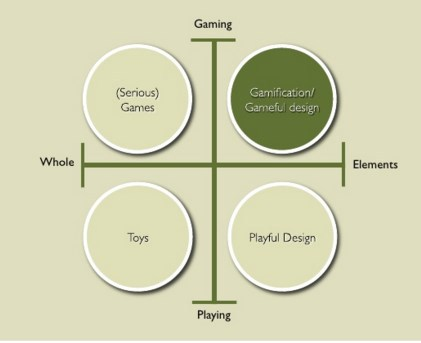
\includegraphics[width=14cm]{chapters/gamification/img/gamification.jpg}
		\caption{A topology of interaction of game-like applications according to its proposes. From \citep{gameAcm} and slightly modified by \cite{gamification_image}.}
		\label{taxonomy}
	\end{center}
\end{figure}


Kelland's definition contributes largely to aims of this research, but, before developing more consistent argues to associate `gamification' and health services, its necessary to explain differences among normal games (toys), serious games, playful design and `gamified' applications. Considering division only of the vertical axis of the figure \ref{taxonomy}, serious games and toys have both a entire narrative or trajectory of playing acts, compounding a whole. On the other hand, a gamified application and an application with playful design are both planed to perform short tasks, in a particular approach. And then considering horizontal axis, on the plan of gaming, gamified application are close to serious games because both are focused on developing intellectual capabilities more the simple joy, as games and toys are.  Colors is an authentic gamified application, but, to simply communication, it is often referred to that as a `game'. The class of gamified applications includes some subtypes. Some authors suggest it can be divided into three subcategories:

\begin{enumerate}
	\item \textbf{Product gamification}: this subtype groups any game-like software designed for attracting the final user in his personal life without a collective or a corporative dimension. That's why it is called \textbf{product} gamification, because it is designed to be used by a single person. Colors' gamification may considered as one of this subcategory.
	\item \textbf{Marketing gamification}: then, when a gamified application targets a entire public of customers, it should be called a process of marketing gamification. The application end is to provide information, brand promotion and satisfaction for potential or usual customers of some enterprise. Today more and more organizations employ this subtype of gamification.
	\item \textbf{Workplace gamification}: finally, some game like-systems are designed to ameliorate working relationships at office. Bonuses, fun challenges and cooperation are general aspects of it. As it will be shown, civil engineering is one of sectors that seems to increase productivity by using of this type of gamification. 
\end{enumerate}

\section{Elements of Gamification}
This process becomes an overused term in computing but sometimes it is applied without the needed scientific rigor. So that it is important to underscore which are the aspect necessary to apply the term to a information system or computational solution. Some of them may be seen as accessory, however, it could sketched a abstract model of gamification essential components. There is also elements that differs the so-called `bad gamification' of simple gaming from the effective gamification, that could be summarized in the following main features \citep{conf/mue/Yamakami13a}:

\begin{enumerate}
	\item  \textbf{Goals}: the player must to have clear objectives to be achieved. On the contrary, the gaming tends to be not useful for constructive purposes and the player's performance never could be measured by a single principle. A gamified application ought to have one general aim in order to be acceptable in such category.
	\item \textbf{Rules}: besides the aforementioned requirement of having at least a single aim, a gamified application requires some valid ways to achieve the goals in opposition to prohibited means. This is possible by a defined set of rules. Generally, gamified applications use to present and teach each one of their rules basing on tutorials, tips and helps. Common games not always follow that point, because sometimes it is interesting for players the process of discovering the rules.
	\item \textbf{Feedback system}: this feature is required only by gamified  application and by serious games in comparing with common or commercial games. The application must check if it has effectiveness targeting its with the public, because it could not be used only by pleasure and be deviated from its original purpose. The feedback process happens both  automatically and by human-made intervention.
	\item \textbf{Voluntary participation}: if a gamified program has obligatory and imposed an aspect  by authorities, the player will not show any compromise with it. Furthermore, the gamification is chosen, as it was said before, to turn boring tasks more pleasant. So, it will a contradiction to impose something designed to transform negative stimuli in positive reception. People could simply prefer return to their functions as they have been designed before the introduction of the pretended gamified application.
\end{enumerate}

The combination of these four characteristics compounds a gamified software. If one of them misses, the application maybe a serious game, a toy or a commercial game, but it could not be classified as a gamified application. These considerations will appear one more time when it was discussed the design of the proposed implementation in the next chapter. The proposed application, \textit{Memory Stroop}, regarded isolate, is a serious game, but when their results are used to check patients' performance by its statistics (whose content is provided by the application proper), it integrates a gamification process, because the gaming will be employed as a mean, as a part of total therapeutic process. Another way to explore gamification essential features is best to show potentials of gamification, as the following figure \ref{taxonomy_1} presents a table with game elements that generally match to human desires (like altruism or reward), suggesting the correlation between gamification demand and its possible uses. 

\begin{figure}[h]
	\begin{center}
		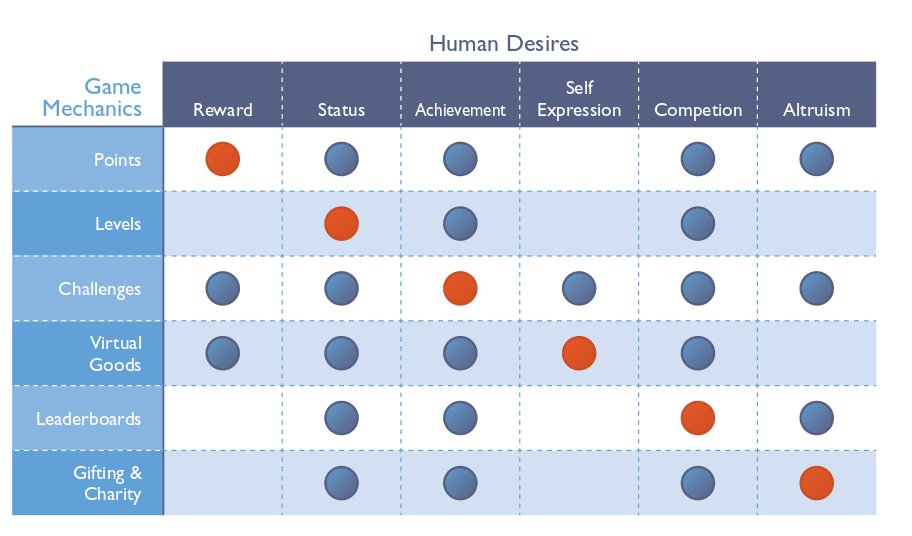
\includegraphics[scale=0.5]{chapters/gamification/img/gaming.jpg}
		\caption{Gaming aspects and human desires \citep{Bunchball}.}
		\label{taxonomy_1}
	\end{center}
\end{figure}

Both approaches are equally useful for the main purposes of this research. Colors apply all of these features in its gaming structure in order to implement a full gamification process. The combination between human desires and gaming features is the mechanism which allows the main aim to bring ADHD diagnosis and treatment more pleasant.


\section{Real Life Cases and Related Work}

Gamification is employed in numerous fields, from construction to psychological therapy. In the case of civil engineering, gamification is part of a deep schema of innovation and investment in technology. By using `gamified' features it's possible to manage activities of labor force, raw materials, plants and other variables of construction, workers can fun themselves with the job without being aside of it. Productivity and satisfaction could be measured from workers' performance in `gamified' ranks  \citep{formoso}. In 2012 the government of Texas, United States, adopted the a gamified system for security monitoring. Before that the Texan public security only monitored the streets by conventional cameras recording activities in streets and by police surveillance, as it is usually performed in all places around the world \citep{conf/cts/Aud13}.

However, after that year introduced a system of security gamification with rewards, rakings and fun-like challenges to reinforce participation of the policemen and of population on monitoring tasks. It was conceived as event-trigger system, by which some criminal occurrence or suspecting acts are regard as a game. Some reduction in violence taxes are registered after that and, according some evidences, this reduction is related with the gamified system \citep{conf/cts/Aud13}. This is a very uncommon use of gamification, that shows the potential offered by that technique. With these basic concepts and instances,  can understand how Gamification systems, independent of its application area, could benefits humans in doing unpleasant or iterative tasks, offering them the possibility of perform these tasks as if they were not `performing' them directly, instead they act as if they are playing a game with real consequences, for example, for its health care.

There is a significant set of scientific works discussing gamification solutions applied to ADHD children. To starts, an article written by Johnstone et al. \citep{Johnstone-2013} evaluates ADHD children neuoral activities along some monitored video gaming sessions and presents evidences that monitored playing. The gamification employed by those articles is based on a specific playing software  that implements the notion of cognitive training, by which cerebral tasks are stimulated continuously and progressively (like the logic of ``levels'' of commercial games) in order to improve child's attention or other mental skills in a almost non-invasive or minimally-invasive way.  Using electrodes in a classical Electro-Cardiogram evaluation in each session, the reduction of concentration deficit's symptoms are statistical significant in their study, what reveals the potential of gamification treatment for ADHD young patients.

Similar method and results are found in another interesting paper \citep{Nemeth}. In fact, that paper is earlier and pioneers some aspects to medical gamification. That work  presents how a therapy by gamification for ADHD children and teenagers may have advantages comparing to drug-centered treatment. They argue that effects of their gaming intervention group has more effective impact and are more permanent than the exclusively psychoactive substances treatment of their control group. So, authors conclude that gaming therapy must gain space in academic studies and, consequently, in clinical psychology. Another space of gamified ADHD child treatment is the school. In this way the work of Izaltino Oliveira \citep{Oliveira}, Brazilian psycho-pedagogue and research, that designed a conceptual model centered in ADHD educational intervention based on gamification. Author says that gamification is one of most powerful tools for younger students in order to develop concentration, mobility and other skills damaged by attention disorder or hyperactivity.

Some authors have stressed relationship of the use of gamified software both for diagnosis and for treatment. It is a total non-invasive method to identifies, and sometime, to treat symptoms related to psychological disorders. There are games of famous corporation like Nintendo, with its NDSBA (Nintendo DS game Brain Age) game among institutions developing brain games directed to hyperactive young people. Unfortunately, so little number of programmers are engaged in this type of medical computing initiative. For that reason, all initiative in this way must be seek anterior work which build new implementations. 

\begin{quote}
However, based on the literature, it seemed feasible that playing brain games such as NDSBA could stimulate the prefrontal cortex of students with ADHD, simulating the effects of stimulant medication, thus helping these students improve their ability to engage in classroom activities and perform tasks of executive function \citep{brainGames}. 
\end{quote}

Letting aside, by now, physiological details, the quotation informs about the importance of gamification in treatment of ADHD. S\'{e}rgio Villa \citeyearpar{Villa}, a Brazilian computer scientist, developed an educational game for android devices and presented it in an undergraduate thesis - both game, Villa's remain paradigmatic to present research.

Villa's game is called in Portuguese ''Cores Beta´´, \textit{Colors} -, which applies Stroop's test principles in order to exercise mental capacities of ADHD children, like low tolerance to frustration. 

As Villa \citeyearpar{Villa} could not develop statistical research with children using his game by himself due difficulties evolving Ethics Committee of Universidade Federal da Bahia -- likewise it happened to the present research --, its necessary to develop and present the computational facilities involving them to check its validity. Different to ordinary games are not projected to this aspect and majority of them may not offer good results for promoting health to the referred children. 

This undergraduate thesis aims to discuss and to present results obtained in practical experiment involving psychologists and computer scientists using principles of ``Cores'' for evaluate its psychotherapy possibilities. All applications proposed for ADHD children up to now do not exploit enough the potential of working memory training. Generally they emphasize the reflexion tasks by which the player must answer to a game assignment correctly in the shorter time as possible. The present application is directed to train memory, not only to measure reaction time to an assignment.


\section{Summary}

In this chapter it was presented the core features, elementary characteristics, finalities and uses of gamification. Briefly it can be described as follows: video game features such as amusing competition and ranking with prizes, gaming levels, playing design, music and so on are used for it purpose. Gamification combines a serious aim, for example a child psycho-pedagogical treatment, with a playing and entertainment framework, what could present more effective results than conventional ways of the serious aim. Almost all daily activities may be treated as at least potential applicable area to gamification. Although gamified systems represent a very recent approach on Information Systems studies, there is a large space of opportunities by using them.

Generally it is seen as a powerful mean to turn heavy tasks into a pleasant design for its agents, this process has a large set of application, from management and finances to health.  Then, it becomes more and more studied and practiced around the world. In the specific case of young patients that suffers with attention and concentration problems gamification may offer a confident and safer alternative to exclusive drug-based treatment \citep{Nemeth}.